\documentclass{llncs}
\usepackage{makeidx}  % allows for indexgeneration
\usepackage[pdftex]{graphicx} % PNGs
\usepackage{amsmath, amssymb} % algebra
\usepackage[utf8x]{inputenc}
\usepackage[T1]{fontenc} 
\usepackage[procnames]{listings} % for sourcecode
\usepackage{graphviz} % graphs
\usepackage{array,multirow} % tables
\usepackage{afterpage} % figures
\usepackage{float} % figures
\usepackage[usenames,dvipsnames]{color}

\restylefloat{figure}
\setlength{\parskip}{0.2em}

% code style
\lstset{
  showstringspaces=true,
  stringstyle=\ttfamily\color{CadetBlue},
  keywordstyle=\color{BurntOrange}\bfseries,
  commentstyle=\color{CadetBlue}\slshape,
  numbers=left,
  numberstyle=\tiny\color{LimeGreen},
  stepnumber=1,
  tabsize=2,
  frame=lines,
  columns=fixed
}

% jaql highlighting
\lstdefinelanguage{jaql}{
  morekeywords={fn,read,write,each,into},
  morecomment=[l]{//},
  literate={->}{$\rightarrow$}{2},
  sensitive=false,
  morestring=[b]",
}

% pig highlighting
\lstdefinelanguage{pig}[]{sql}{
  sensitive=true
}

\begin{document}
  
  \pagestyle{headings}  % switches on printing of running heads
  %\mainmatter % start of the contributions
  \title{Hadoop Scripting Languages}
  \subtitle{Domain Specific Languages Pig and Jaql}
  \titlerunning{Hadoop Scripting}  % abbreviated title (for running head)
  \author{Johan Uhle, Konstantin Haase}
  \date{\today}
  \authorrunning{Uhle, Haase}   % abbreviated author list (for running head)
  \tocauthor{Johan Uhle, Konstantin Haase (Hasso-Plattner-Institute)}
  \institute{Seminar ``Map/Reduce Algorithms on Hadoop'',\\
    Research Group Information Systems,
    Alexander Albrecht, Prof. Felix Naumann,
    Hasso-Plattner-Institut, Universität Potsdam,
    D-14482 Potsdam, Germany,\\
    \email{\{johan.uhle, konstantin.haase\}@student.hpi.uni-potsdam.de}}
  
  \maketitle
  
  \begin{abstract}  
In this paper the domain specific languages Pig and Jaql for Map/Reduce on Hadoop~\cite{hadoopWebsite} are compared regarding their features, ease of programming and speed.
\end{abstract}   
  
  \section{Introduction}

Working with big data sets has gained growing significance in the past years. This means processing heterogenous Gigabytes or terabytes of plain text by filtering, grouping or applying functions on the whole set or elements. One solution to this problem is using the Map/Reduce paradigm, which enables a cluster of computers to process a problem parallel and thus increase the processing speed.

Apache Hadoop is an Open Source Implementation of Map/Reduce. It is published under the Apache License and is maintained by the Apache Foundation. It's development is mostly driven by Yahoo! employers.

Hadoop programs are written in Java against the Hadoop API. On top of Hadoop, several domain specific languages try to establish a more abstract approach to the Map/Reduce paradigm. We have chosen Pig and Jaql to compare them in feature set, ease of programming and processing speed.

All source code written in running the benchmarks for this paper are published at GitHub under Apache License \footnote{available at http://github.com/rkh/hadoop-scripting/}.            % johan
  \section{Jaql}

Jaql~\cite{jaqlWebsite} is a high-level scripting language for the JavaScript Object Notation (JSON).
It is able to run on Hadoop and break most requests down to Map/Reduce tasks.
Jaql heavily borrowes from SQL, XQuery, LISP, Pig Latin, JavaScript and Unix Pipes.~\cite{jaqlOverview}

Developed mainly inside IBM and with a quite mailinglist Jaql currently faces
a serious lack of documentation and community. The documentation found online
is outdated and incomplete in most cases. In addition, Jaql was undergoing
major changes in the time of writing this paper.

Even though available, there is no need to write in a strict Map/Reduce pattern. At the point of execution (i.e. the end of a query statement) Jaql transforms the
parsed statement into another, equivalent but optimised statement. This step is
comparable to a query optimiser in modern database management systems. The optimised
query can in turn be transformed back to Jaql code, which is useful for debugging.

Jaql can be extended with user-defined functions, written either in Java or
in Jaql itself. However, it is not possible to use Jaql as a general-purpose programming
language, as it is not Turing-complete: It lacks both recursion and a universal loop
function.

The current Jaql implementation features three modes to run in: In stand-alone mode Hadoop
is not used at all and the jobs are not split in Map/Reduce tasks. When using Jaql
with Hadoop a so-called mini-cluster can be used, which is managed by Jaql and runs all tasks
on one computer in the same process (with one thread per Map/Reduce task), or an external hadoop cluster.                    % konstantin
  \section{Pig}

Pig~\cite{pigWebsite} is a high level scripting language for data transformation. It is a Hadoop Subproject and in the Apache Incubator since 2007. Just as Hadoop it is mainly developed by Yahoo!, where in early 2009 30 \% of all Map/Reduce jobs have been implemented using Pig.~\cite{pig30percent}

It has an active community and a growing ecosystem. \footnote{http://hadoop.apache.org/pig/mailing_lists.html}

The development of Pig took three key aspects into account. ~\cite{pigWebsite} \\
The \emph{ease of programming} enables the user to create powerful scripts that are easy to write, read and maintain against very large data sets.

\emph{Optimisation} was another goal. When writing a Pig script, it is not needed for the programmer to think within the Map/Reduce paradigm since Pig handles the transformation of the script to the particular Map/Reduce jobs. This also offers opportunities for automatic optimisations made by the Pig compiler. A good explanation about how Pig parses and compiles a Pig script can be found in the paper ``Pig Latin: A Not-So-Foreign Language for Data Processing'' Chapter 4.~\cite{pigNotForeign}

Pig features \emph{extensibility} achieved by user-defined functions which are programmed in Java against the Pig interfaces and may be called within Pig Latin. Thus Pig has the same feature set as Java Hadoop.

Pig uses the scripting language Pig Latin~\cite{pigManual}. The syntax looks similar to SQL (which may be integrated into Pig additionally~\cite{pigSql}), albeit Pig Latin is a data transformation language and therefore works similar to the database query optimiser in modern database management systems.

Pig Latin Scripts often do not consist of more than 10 lines of code, whereas user-defined functions in Java are more complex and may need more than 100 lines of code.
                                                                                                                                    % johan
  \section{Cluster Setup}

All benchmarks were measured on the same cluster consisting of ten nodes. Unfortunately our nodes did vary in hardware widely, especially in CPU and memory. Two of the nodes were two upto four times faster than the others. This caused some variation in performance tests when running with a small number of map or reduce tasks, since the workload of the faster nodes varied depending on how many tasks they have got assigned. In our opinion a homogenous cluster would be more suited for benchmarking. We used Hadoop version 0.18.3 since neither Pig nor Jaql are compatible with the current version of Hadoop (0.20). We ran the latest version of Pig 0.3.0 and a development snapshot of the upcoming Jaql 0.4\footnote{available at http://github.com/rkh/jaql}. During the Markov Chain benchmarks we also tried Jaql 0.3 and both release candidates for Jaql 0.4.                 % konstantin
  \section{Scenario: Wordcount}

In the following wordcount scenario the words in a document are counted by number of occurrence. This scenario fits the purpose of comparing the different approaches very well, because counting words is a classic Map/Reduce task. Furthermore programming a wordcount script is fairly easy and therefore limits the impact of our programming skills against the benchmark results.      % johan
  %\clearpage
\section{Benchmark: Wordcount}           

We have been running our Hadoop Java, Pig and Jaql scripts against a series of Wikipedia articles with a sizes between 10 Mb and 5000 Mb and 4 runs for each size.

\begin{figure}[H]
  \begin{center}
    \includegraphics[width=\textwidth]{../benchmarks/wordcount}
  \end{center}
  \caption{Wordcount performance benchmark results}
  \label{fig:reducers}
\end{figure}

It can be observed that Java performes better by an order of magnitude, compared to Pig and Jaql, which do not differ that much from each other. Apparently all do scale well, since execution time is growing slower than input size for all three implementations.    % johan
  %\section{Scenario: Markov Chain} 

We split text into word tuples with key words and successor.

The code used for benchmarking is available under Apache License at Github. \footnote{available at http://github.com/rkh/hadoop-scripting/}        % konstantin
  \section{Programming with Jaql}

\begin{lstlisting}[language=jaql,caption=A sample Jaql query,label=jaqlsample]
$source = "http://server/api.php?format=json\&query=foo";
read(http($source)) 
  -> transform each $["name"]
  -> write(hdfs("output.dat"));
\end{lstlisting}

One of the main features of Jaql is the ability to read from and write to different
storage types, currently the local file system, the Hadoop Distributed File System,
HBase and HTTP. Since Jaql is based on JSON, reading
from HTTP allows easy integration of web services like Wikipedia or Flickr, that offer
a JSON API.

A typical Jaql request can be seen in listing \ref{jaqlsample}. Jaql ships with an
interactive shell (read-eval-print loop). 

Jaql features two ways of passing parameters to a function. You can write the parameters
in brackets after the function name, as known from most other programming languages, i.e.
\lstinline[language=jaql]!foo("bar")!. However, Jaql also features a new pipe syntax, more
consistent with the way built in Jaql statements are written. The value you ``pipe into''
a function will be past as the first argument, therefore \lstinline[language=jaql]!foo("bar", "baz")!
is equivalent to \lstinline[language=jaql]!"bar" -> foo("baz")!.

All values, either arguments or return values, are JSON objects or Jaql functions.
Every function in Jaql returns a value. Jaql offers advanced functionality for querying, transforming
and aggregating those values. An example can be seen in listing \ref{jaqlwc}. Note that
operations like {\tt expand} or {\tt group by} will loop through all element of the given array
and potentially split this operation on multiple Map/Reduce tasks. Within a loop {\tt\$} is referring
to the current element.

\begin{lstlisting}[language=jaql,caption=Wordcount in Jaql,label=jaqlwc]
read($src)
  -> expand splitArr($, " ")
  -> group by $w = ($) into [$w, count($)];
\end{lstlisting}

A statement is terminated by a semicolon and will at that point be optimized, as mentioned earlier.
However, instead of executing the statement, Jaql is able to return the optimized Jaql code by calling
{\tt explain} on the statement.   % konstantin
  \section{Programming With Pig}

For using Pig, two ways are possible. One is Grunt, an interactive Shell for Pig. The other way is evaluating an external script with Pig. Both ways work in localmode (Pig standalone) and in Hadoop Mode.
                              
A typical Pig Latin line of code looks like listing \ref{pigsample}.

\begin{lstlisting}[language=pig,caption=A typical Pig line of code,label=pigsample]
ordered = ORDER words;
\end{lstlisting}

This is the data transformation of one set (``words'') with an operation (``ORDER'') into a new set (``ordered''). The input data sets are always on the right side of the equation. The resulting output data set is always on the left side.

Most often Pig Latin Scripts naturally follow this listings structure \ref{pigstructure}.

\begin{lstlisting}[language=pig,caption=Pig Latin Script Structure ,label=pigstructure]
Load Data -> Manipulate Data -> Group Data -> Output Data
\end{lstlisting}
                                                       
A Pig Latin script is always started by a {\tt LOAD} statement. The loaded is manipulated via {\tt FILTER}, {\tt FOREACH ... GENERATE} or {\tt DISTINCT} statements or with the help of user-defined functions. Afterwards the Data gets grouped. Then the cycle either starts all over again e.g. with additional data being joined or the resulting data set is written to the output with a STORE statement. Of course this structure is not compulsory.
                   
Every data set has a schema determining the structure of the data. These schemas may be defined explicitly by the user in Pig Latin or in a UDF or implicitly by Pig. Certain attributes in a data set are to be accessed either via the corresponding name in the schema or via position.
As already stated Pig has the same possibilities as native Java Hadoop due to the use of user-defined functions (UDF \ref{pigudf}). These functions may implement custom load or store functionality or manipulate per element or over a whole data set. It is also possible to use UDFs for filtering by deciding if certain data shall be in the resulting data set or not.
The development of UDFs is well documented but requires noteworthy more effort than just writing Pig Latin. Especially defining own schemas can be a hard-to-debug task. 

Pig Latin scripts are best to debugged with the {\tt ILLUSTRATE}, {\tt DESCRIBE} and {\tt DUMP} statements, which are giving access to the schema and the data of the data sets. Unfortunately schemas are only to be viewed one level deep and therefor deeper nested data structures are hard to debug.    % johan
  %\section{Benchmark: Markov Chain}

\begin{figure}[tb]
  \begin{center}
    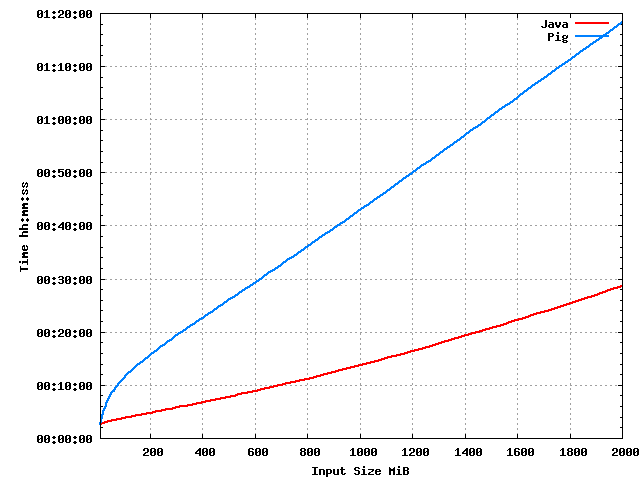
\includegraphics[width=\textwidth]{../benchmarks/markov}
  \end{center}
  \caption{Markov Chain benchmark results}
  \label{fig:reducers}
\end{figure}

We have been running a Hadoop Java and a Pig implementation on the cluster against a series of Wikipedia articles with a size of 10 Mb to 2000 Mb. To minimise benchmark errors we have done 4 runs for each size.

It is clearly visible, that Pig is slower than the native Java implementation.       % johan
  \section{Conclusion}

Both Pig and Jaql ease programming for Hadoop by allowing rapid development, compared to Hadoop's
Java interface. They are both in an early stage of development and cannot yet fully compete with
pure Java performance in our macro benchmarks.              % konstantin 

  %
%  \section{Lessons learned}
%  \begin{figure}[tb]
%    \begin{center}
%      %\includegraphics{reducers}
%    \end{center}
%    \caption{Processing Speed in Relation to Number of Reducers}
%    \label{fig:reducers}
%  \end{figure} 
  
  %\nocite{*}
  \bibliographystyle{splncs}
  %\bibliographystyle{authordate1}
  \bibliography{hadoop}
  \clearpage
\end{document}
